\documentclass[11pt,twoside,a4paper]{article}
\usepackage[utf8]{inputenc}
\usepackage[spanish]{babel}
\usepackage[margin=2.5cm]{geometry}
\usepackage{amsmath}
\usepackage{amssymb}
\usepackage{listings}
\usepackage{xcolor}
\usepackage{fancyhdr}
\usepackage{hyperref}
\usepackage{graphicx}
\usepackage{float}

% Configuración de headers
\pagestyle{fancy}
\fancyhf{}
\lhead{\small\textit{Procesamiento de Datos en Series Temporales}}
\rhead{\thepage}

% Colores para código
\definecolor{codeblue}{RGB}{30, 136, 229}
\definecolor{codegreen}{RGB}{67, 160, 71}
\definecolor{codealert}{RGB}{229, 57, 53}

% Configuración de listings
\lstset{
    language=Python,
    basicstyle=\ttfamily\small,
    commentstyle=\color{gray}\itshape,
    keywordstyle=\color{codeblue}\bfseries,
    stringstyle=\color{codegreen},
    breaklines=true,
    breakatwhitespace=true,
    tabsize=4,
    numbers=left,
    numberstyle=\tiny\color{gray},
    stepnumber=1
}

% Comandos personalizados
\newcommand{\code}[1]{\texttt{\small #1}}
\newcommand{\eq}[1]{\textbf{(#1)}}

\title{\Large\textbf{Procesamiento de Datos en Series Temporales Multimodales} \\
       \normalsize Reference Guide Técnica --- FatigueSet Biometría}
\author{Análisis de Windowing, Data Leakage, Sincronización y Normalización}
\date{2026}

\begin{document}

\maketitle

\section*{Aviso}
\noindent Documento técnico que sintetiza el análisis práctico de los notebooks:
\begin{itemize}
    \item \code{windowing\_data\_leakage.ipynb}
    \item \code{sincronizacion\_normalizacion.ipynb}
\end{itemize}
Incluye espacios designados \texttt{[IMG]} para inserción de figuras principales.

\newpage
\tableofcontents
\newpage

% ============================================================
% INTRODUCCIÓN
% ============================================================
\section{Introducción}

El procesamiento de datos de series temporales multimodales en biometría es una tarea crítica para:
\begin{enumerate}
    \item Evitar artefactos y ruido estructural
    \item Prevenir \textbf{data leakage}: contaminación información train $\leftrightarrow$ test
    \item Sincronizar sensores que operan a distintas frecuencias
    \item Normalizar correctamente sin sesgos
\end{enumerate}

Este documento proporciona:
\begin{itemize}
    \item \textbf{Teoría}: Ecuaciones formales y conceptos fundamentales
    \item \textbf{Práctica}: Código Python y pseudocódigo ejecutable
    \item \textbf{Datos reales}: Valores del dataset FatigueSet (12 sujetos, 3 sesiones)
\end{itemize}

\noindent\textbf{Nota}: Los ejemplos numéricos provienen directamente de ejecuciones en los notebooks referenciados.

% ============================================================
% CAPÍTULO 1: CONCEPTOS FUNDAMENTALES
% ============================================================
\section{Conceptos Fundamentales}

\subsection{Series Temporales en Biometría}

Una serie temporal es una secuencia de observaciones ordenadas en el tiempo:
\begin{equation}
\mathbf{x} = [x_1, x_2, \ldots, x_n] \quad \text{donde} \quad x_t \in \mathbb{R}, \quad t \in \{1,\ldots,n\}
\end{equation}

En biometría multimodal, se adquieren \textbf{múltiples señales simultáneamente}:

\begin{table}[H]
\centering
\caption{Sensores en FatigueSet (P01/S01 --- 26.3 minutos)}
\label{tab:sensores}
\begin{tabular}{|l|r|r|r|}
\hline
Sensor & Filas & Hz estimado & Duración (min) \\
\hline
Chest HR (Zephyr) & 1578 & 1.00 & 26.3 \\
\hline
EDA (Empatica E4) & 6313 & 4.00 & 26.3 \\
\hline
EEG Alpha (Muse) & 14400 & 9.13 & 26.3 \\
\hline
\end{tabular}
\end{table}

\textbf{Problema fundamental}: Aunque todas duran 26.3 minutos, cada sensor opera con su propio reloj interno. El índice de fila $i$ en cada señal \textit{no corresponde al mismo instante temporal}. Esto requiere sincronización explícita.

\subsection{Frecuencia de Muestreo y Aliasing}

La frecuencia de muestreo es el número de muestras por segundo:
\begin{equation}
f_s = \frac{\text{número de muestras}}{\text{duración en segundos}}
\end{equation}

Según el teorema de Nyquist, la frecuencia máxima que puede capturarse sin aliasing es $f_s / 2$.

Implicación: Si EEG se muestrea a $\approx 256$ Hz, pero downsampling a 1 Hz descardaría frecuencias $> 0.5$ Hz. Para señales fisiológicas (variabilidad cardiaca, ritmos cerebrales) esto puede ser problemático.

% ============================================================
% CAPÍTULO 2: WINDOWING Y FEATURE EXTRACTION
% ============================================================
\section{Windowing y Extracción de Features}

\subsection{Definición Formal}

Windowing divide una serie temporal de longitud $n$ en $m$ segmentos de tamaño $k$:

\begin{equation}
W_i = \{x_j : \text{inicio}_i \leq j < \text{inicio}_i + k\}, \quad i = 1, \ldots, m
\end{equation}

donde el inicio de cada ventana es:
\begin{equation}
\text{inicio}_i = i \cdot \text{step\_size}
\end{equation}

El número de ventanas resultantes:
\begin{equation}
m = \left\lfloor \frac{n - k}{\text{step\_size}} \right\rfloor + 1
\end{equation}

Cada ventana se transforma en \textbf{features escalares} (estadísticos):
\begin{align}
\mu_i &= \frac{1}{k} \sum_{j \in W_i} x_j \quad \text{(media)} \\
\sigma_i &= \sqrt{\frac{1}{k} \sum_{j \in W_i} (x_j - \mu_i)^2} \quad \text{(desviación)} \\
\text{min}_i &= \min(W_i), \quad \text{max}_i = \max(W_i) \quad \text{(extremos)}
\end{align}

\subsection{Sliding sin Solapamiento vs Con Solapamiento}

\subsubsection{Sin solapamiento}
\begin{equation}
\text{step\_size} = k \implies m = \lfloor n / k \rfloor
\end{equation}

Las ventanas son disjuntas. Con $n=1578$ muestras y $k=100$: $m = 15$ ventanas.

\subsubsection{Con solapamiento}
\begin{equation}
\text{step\_size} < k \implies m = \left\lfloor \frac{n - k}{\text{step\_size}} \right\rfloor + 1
\end{equation}

Con $k=100$ y $\text{step\_size}=50$ (50\% overlap): $m = 30$ ventanas ($2\times$ más).

\textbf{Trade-off}:
\begin{itemize}
    \item Sin overlap: Menos muestras, pero sin correlación espuria
    \item Con overlap: Más muestras, pero alta correlación temporal entre ventanas consecutivas
\end{itemize}

El solapamiento introduce un riego crítico si el split train/test es \textbf{aleatorio}: los datos correlacionados pueden filtrarse mutuamente. Esto es \textbf{data leakage}.

\subsection{Pseudocódigo: Crear Ventanas}

\begin{lstlisting}[caption=Algoritmo de windowing]
def crear_ventanas(serie, window_size, step_size):
    """Segmenta serie temporal en ventanas."""
    ventanas = []

    for inicio in range(0, len(serie) - window_size + 1, step_size):
        fin = inicio + window_size
        ventana = {
            'indices': (inicio, fin),
            'timestamp_inicio': timestamps[inicio],
            'timestamp_fin': timestamps[fin - 1],
            'valores': serie[inicio:fin]
        }
        ventanas.append(ventana)

    return ventanas

# Ejemplo
n_ventanas = crear_ventanas(hr_data, window_size=100, step_size=50)
print(f"Total ventanas: {len(n_ventanas)}")
\end{lstlisting}

% ============================================================
% CAPÍTULO 3: DATA LEAKAGE
% ============================================================
\newpage
\section{Data Leakage: Cuatro Fuentes de Contaminación}

Data leakage ocurre cuando \textbf{información del conjunto de test filtra al modelo durante entrenamiento}, invalidando validación experimental.

\subsection{Leakage 1: Split Temporal Incorrecto}

\subsubsection{El Problema}

En series temporales, un split \textbf{aleatorio} mezcla pasado y futuro:

\begin{equation}
\text{Aleatorio (MAL)}: \quad \text{train} = \{W_1, W_3, W_4, \ldots\}, \quad \text{test} = \{W_2, W_5, \ldots\}
\end{equation}

Si train contiene indicador posterior a test, el modelo "conoce el futuro".

\subsubsection{La Solución}

Split \textbf{temporal} con límite claro:

\begin{equation}
\text{Split en } t_c: \quad \text{train} = \{(t_i, x_i) : t_i < t_c\}, \quad \text{test} = \{(t_i, x_i) : t_i \geq t_c\}
\end{equation}

Además, hacer windowing \textbf{después del split}, no antes.

\subsubsection{Resultados Cuantitativos}

En P01/S01 con 30 ventanas (overlap 50\%) y split aleatorio:
\begin{itemize}
    \item \textbf{95.8\%} de ventanas train inician después de la primera ventana test
    \item Contaminación severa: información temporal entrelazada
\end{itemize}

Split temporal correcto (en índice 1262 de 1578):
\begin{itemize}
    \item Train: 24 ventanas, Test: 5 ventanas
    \item \textbf{0\%} de solapamiento de índices entre folds
\end{itemize}

\subsection{Leakage 2: Normalización Global}

\subsubsection{El Problema}

Normalización Z-score típica calcula media y desviación con \textbf{todos los datos}:

\begin{equation}
\mu_{\text{ALL}} = \frac{1}{N_{\text{total}}} \sum_{i=1}^{N_{\text{ALL}}} x_i
\end{equation}

Esto incluye test. Resultado: información de test contamina el normalizador.

\subsubsection{La Solución}

Calcular estadísticas \textbf{solo con datos de entrenamiento}:

\begin{equation}
\mu_{\text{TRAIN}} = \frac{1}{n_{\text{train}}} \sum_{i \in \text{TRAIN}} x_i, \quad
\sigma_{\text{TRAIN}} = \sqrt{\frac{1}{n_{\text{train}}} \sum_{i \in \text{TRAIN}} (x_i - \mu_{\text{TRAIN}})^2}
\end{equation}

Luego normalizar ambos conjuntos:

\begin{equation}
z_i = \frac{x_i - \mu_{\text{TRAIN}}}{\sigma_{\text{TRAIN}}} \quad \forall i \in \text{TRAIN} \cup \text{TEST}
\end{equation}

\subsubsection{Impacto Cuantitativo}

Comparando normalización global vs train-only en FatigueSet:

\begin{table}[H]
\centering
\caption{Diferencia en valores test normalizados: global vs train-only}
\label{tab:leakage_norm}
\begin{tabular}{|l|r|}
\hline
Feature & $|\Delta|$ promedio \\
\hline
max & 0.0387 \\
\hline
std & 0.0360 \\
\hline
mean & 0.0348 \\
\hline
range & 0.0332 \\
\hline
min & 0.0125 \\
\hline
\end{tabular}
\end{table}

Aunque pequeño individualmente, acumula error en 100+ muestras.

\subsection{Leakage 3: Overlapping + Split Aleatorio}

\subsubsection{El Problema}

Con solapamiento alto ($\text{step} \ll k$), ventanas consecutivas comparten $> 50\%$ índices:

\begin{equation}
W_i = [x_1, \ldots, x_{100}], \quad W_{i+1} = [x_{51}, \ldots, x_{150}]
\end{equation}

Si split es aleatorio, train y test comparten esos 50 índices comunes.

\subsubsection{Similitud Coseno}

La similitud coseno entre dos vectores mide su alineación:

\begin{equation}
\text{sim}(\mathbf{u}, \mathbf{v}) = \frac{\mathbf{u} \cdot \mathbf{v}}{|\mathbf{u}| \cdot |\mathbf{v}|}
\end{equation}

Valores: $[-1, 1]$ (típicamente $[0, 1]$ para datos no-negativos).

\subsubsection{Resultados}

En P01/S01:
\begin{itemize}
    \item Split aleatorio: similitud máxima $\approx 0.9979$, solapamiento $\approx 50\%$
    \item Split temporal post-windowing: similitud $\approx 0.9983$, solapamiento $\approx 50\%$ (frontera contaminada)
    \item Split temporal correcto: similitud $\approx 0.9979$, solapamiento $= 0\%$ (sin contaminación)
\end{itemize}

\textbf{Conclusión}: El solapamiento de índices es más crítico que la similitud coseno.

\subsection{Leakage 4: Entre Sujetos (LOSO)}

\subsubsection{El Problema}

En biometría, si el mismo sujeto aparece en train y test, el modelo aprende \textbf{identidad} (quién es) en lugar de \textbf{estado} (cómo está: fatiga, estrés).

\subsubsection{La Solución: Leave-One-Subject-Out}

Para cada sujeto $p$:

\begin{equation}
\text{FOLD}_p: \quad \text{TRAIN}_p = \{x_i : s_i \neq p\}, \quad \text{TEST}_p = \{x_i : s_i = p\}
\end{equation}

Esto valida que el modelo generaliza a \textbf{nuevos sujetos} sin datos previos.

\subsubsection{Correctitud en LOSO}

Si usamos normalización por-sujeto en LOSO:

\begin{equation}
\mu_p^{\text{TRAIN}} = \frac{1}{n_p^{\text{TRAIN}}} \sum_{i \in \text{TRAIN}, s_i=p} x_i
\end{equation}

La media $\mu_p$ se calcula \textbf{solo con datos del fold de entrenamiento}, nunca test.

Véase Tabla \ref{tab:loso_sim}: simulación LOSO en FatigueSet (108 filas = 12 sujetos $\times$ 9 muestras/sujeto).

\begin{table}[H]
\centering
\caption{Distribución LOSO: puntos por fold}
\label{tab:loso_sim}
\begin{tabular}{|r|r|r|}
\hline
Sujeto Test & n\_train & n\_test \\
\hline
Cualquiera & 99 & 9 \\
\hline
\end{tabular}
\end{table}

\subsection{Checklist Anti-Leakage}

Antes de entrenar, verificar:

\begin{enumerate}
    \item[$\checkmark$] \textbf{Split antes de windowing}: Dividir datos brutos en train/test por tiempo/sujeto primero

    \item[$\checkmark$] \textbf{Normalización train-only}: $\mu, \sigma$ calculadas \textbf{solamente} del conjunto entrenamiento

    \item[$\checkmark$] \textbf{Evitar overlap train-test}: Verificar que no hay solapamiento de índices entre folds

    \item[$\checkmark$] \textbf{Features sin visión al futuro}: Ningún feature depende de valores posteriores a su ventana

    \item[$\checkmark$] \textbf{LOSO para biometría}: Validar con leave-one-subject-out, no random cross-validation

    \item[$\checkmark$] \textbf{Recalcular normalizadores por fold}: Cada fold en LOSO tiene sus propios $\mu, \sigma$ de TRAIN
\end{enumerate}

% ============================================================
% CAPÍTULO 4: SINCRONIZACIÓN MULTIMODAL
% ============================================================
\newpage
\section{Sincronización Multimodal}

\subsection{El Problema de los Relojes Distintos}

Cada sensor registra timestamps independientes:

\begin{lstlisting}
# Chest HR - 1 muestra/segundo
t_chest = [10:53:43, 10:53:44, 10:53:45, ...]

# EDA - 4 muestras/segundo
t_eda = [10:53:43.00, 10:53:43.25, 10:53:43.50, ...]

# EEG - ~256 Hz
t_eeg = [10:53:43.0039, 10:53:43.0078, 10:53:43.0117, ...]
\end{lstlisting}

Los \textbf{índices de fila no son equivalentes} entre sensores. Índice 100 en HR $\neq$ índice 100 en EDA $\neq$ índice 100 en EEG.

\subsection{Pipeline de Sincronización}

La sincronización requiere 5 pasos:

\begin{enumerate}
    \item \textbf{Indexar por datetime}: Usar timestamp como índice, no número de fila
    \item \textbf{Elegir frecuencia objetivo}: Tipicamente, la del sensor más lento
    \item \textbf{Resampling}: Cambiar la frecuencia de cada señal
    \item \textbf{Interpolación}: Rellenar valores faltantes
    \item \textbf{Concatenación}: Fusionar en tensor 2D sincronizado
\end{enumerate}

\textbf{Frecuencia objetivo en FatigueSet}: 1 Hz (dictada por HR del chest, el más lento).

\subsection{Resampling}

\subsubsection{Downsampling}

Reducir Hz mediante agregación (típicamente media):

\begin{equation}
y[t] = \text{MEAN}(\{x[t + k \cdot \Delta t] : k = 0, 1, \ldots, m\})
\end{equation}

Ejemplo: EDA de 4 Hz a 1 Hz

\begin{table}[H]
\centering
\caption{Downsampling EDA: 4 Hz $\to$ 1 Hz}
\label{tab:downsample}
\begin{tabular}{|l|r|}
\hline
Original & 6313 muestras \\
\hline
Downsampled (1 Hz) & 1578 muestras \\
\hline
Ratio reducción & $\approx 4\times$ \\
\hline
\end{tabular}
\end{table}

\subsubsection{Upsampling}

Aumentar Hz creando posiciones temporales vacías (NaN):

\begin{lstlisting}
# Pseudocodigo
hr_original = [70, 72, 65, 68, ...]  # 1 muestra/s
hr_250ms = [70, NaN, NaN, NaN, 72, NaN, NaN, NaN, 65, ...]
# 4 muestras/s: 3 NaN nuevos por cada valor original
\end{lstlisting}

En FatigueSet, upsampling HR de 1 Hz a 250 ms (4 Hz):

\begin{table}[H]
\centering
\caption{Upsampling HR: 1 Hz $\to$ 250 ms (4 Hz)}
\label{tab:upsample}
\begin{tabular}{|l|r|}
\hline
Original & 1578 muestras \\
\hline
Upsampled (250ms) & 6309 posiciones \\
\hline
Valores conocidos & 1578 \\
\hline
NaN generados & 4731 (75.0\%) \\
\hline
\end{tabular}
\end{table}

\subsection{Interpolación}

Las posiciones vacías (NaN) deben rellenarse. Métodos comunes:

\subsubsection{A) Interpolación Lineal}

Conecta puntos conocidos con recta:

\begin{equation}
y_{\text{interp}}[t] = y[t_i] + \frac{t - t_i}{t_{i+1} - t_i} (y[t_{i+1}] - y[t_i])
\end{equation}

Donde $t_i \leq t < t_{i+1}$ son dos timestamps adyacentes con valores.

\subsubsection{B) Interpolación Spline Cúbica}

Usa polinomios cúbicos por tramos, garantizando continuidad $C^2$:

\begin{equation}
y_{\text{spline}}(t) = a_i + b_i(t - t_i) + c_i(t - t_i)^2 + d_i(t - t_i)^3
\end{equation}

para $t \in [t_i, t_{i+1}]$.

\subsubsection{C) Forward Fill (Zero-Order Hold)}

Mantiene el último valor:

\begin{equation}
y_{\text{ffill}}[t] = y[t_i] \quad \text{para todo} \quad t \in [t_i, t_{i+1})
\end{equation}

Útil para eventos discretos; introduce escaleras en señales continuas.

\subsubsection{Comparación Empírica}

En HR upsampled (5 minutos):

\begin{table}[H]
\centering
\caption{Métodos interpolación: características}
\label{tab:interp_comp}
\begin{tabular}{|l|l|}
\hline
\textbf{Método} & \textbf{Propiedad} \\
\hline
Lineal & Cambios de pendiente abruptos \\
\hline
Spline & Curva suave, natural \\
\hline
Forward fill & Escaleras; para eventos discretos \\
\hline
\end{tabular}
\end{table}

\textbf{Usaremos}: Spline cúbica para señales fisiológicas continuas.

\subsection{Pipeline Completo}

\begin{lstlisting}[caption=Pipeline sincronización multimodal]
FREQ_OBJETIVO = '1s'  # 1 Hz

def sincronizar_senal(dataframe, columna, freq=FREQ_OBJETIVO):
    # 1. Indexar por datetime
    ts = dataframe.set_index('datetime')[columna]\
                  .sort_index().dropna()

    # 2. Resampling a frecuencia objetivo
    resampled = ts.resample(freq).mean()

    # 3. Interpolacion + ffill para rellenos finales
    interpolated = resampled.interpolate('linear')\
                            .ffill().bfill()

    return interpolated

# Aplicar a cada sensor
hr_sync = sincronizar_senal(df_chest, 'hr')
eda_sync = sincronizar_senal(df_wrist, 'eda')
eeg_mean = df_eeg[CANALES_EEG].mean(axis=1)
eeg_sync = sincronizar_senal(df_eeg_con_media, 'eeg_mean')

# 4. Concatenacion en tensor sincronizado
tensor = pd.concat([hr_sync, eda_sync, eeg_sync],
                    axis=1).dropna()

# Resultado: [T x 3] donde T = 1578 instantes
print(f"Tensor: {tensor.shape}")  # (1578, 3)
\end{lstlisting}

\subsubsection{Resultado del Tensor}

\begin{table}[H]
\centering
\caption{Ejemplo tensor sincronizado (10 filas)}
\label{tab:tensor}
\begin{tabular}{|l|r|r|r|}
\hline
\textbf{Timestamp} & \textbf{HR (bpm)} & \textbf{EDA ($\mu$S)} & \textbf{EEG alpha (dB)} \\
\hline
2021-08-19 10:53:43 & 64.0000 & 0.0705 & 0.4308 \\
\hline
2021-08-19 10:53:44 & 62.0000 & 0.0695 & 0.4114 \\
\hline
2021-08-19 10:53:45 & 59.0000 & 0.0705 & 0.2709 \\
\hline
2021-08-19 10:53:46 & 59.0000 & 0.0698 & 0.2819 \\
\hline
\vdots & \vdots & \vdots & \vdots \\
\hline
\end{tabular}
\end{table}

Ahora cada fila corresponde al mismo instante temporal para las tres modalidades.

% ============================================================
% CAPÍTULO 5: NORMALIZACIÓN
% ============================================================
\newpage
\section{Normalización de Datos}

\subsection{Normalización Global}

\subsubsection{Definición}

Z-score calculado sobre \textbf{todo el dataset}:

\begin{equation}
\mu_{\text{global}} = \frac{1}{N} \sum_{i=1}^{N} x_i
\end{equation}

\begin{equation}
\sigma_{\text{global}} = \sqrt{\frac{1}{N} \sum_{i=1}^{N} (x_i - \mu_{\text{global}})^2}
\end{equation}

\begin{equation}
z_i^{\text{global}} = \frac{x_i - \mu_{\text{global}}}{\sigma_{\text{global}}}
\end{equation}

\subsubsection{Interpretación}

Mantiene \textbf{diferencias basales entre individuos}. La información de nivel fisiológico permanece codificada.

Ejemplo: HR en reposo (Persona A: 55 bpm vs Persona B: 85 bpm).

Con $\mu_{\text{global}} = 87.88$ bpm, $\sigma_{\text{global}} = 20.16$:

\begin{align}
z_A &= \frac{55 - 87.88}{20.16} = -1.63 \\
z_B &= \frac{85 - 87.88}{20.16} = -0.14
\end{align}

La diferencia relativa permanece: $\Delta z \approx 1.5$.

\subsubsection{Ventajas y Riesgos}

\begin{table}[H]
\centering
\caption{Normalización global: trade-offs}
\label{tab:norm_global_trade}
\begin{tabular}{|l|l|}
\hline
\textbf{Ventajas} & \textbf{Riesgos} \\
\hline
Mantiene diferencias inter-sujeto & Modelo aprende identidad \\
\hline
Generaliza a nuevos sujetos & Sensible a outliers \\
\hline
Escala única & Confunde "quién" con "cómo" \\
\hline
\end{tabular}
\end{table}

\subsubsection{Resultados en FatigueSet}

Parámetros globales (108 filas \texttimes\ 3 features):

\begin{table}[H]
\centering
\caption{Estadísticas normalización global}
\label{tab:norm_global_params}
\begin{tabular}{|l|r|r|}
\hline
Feature & $\mu_{\text{global}}$ & $\sigma_{\text{global}}$ \\
\hline
HR (bpm) & 87.8750 & 20.1570 \\
\hline
EDA ($\mu$S) & 1.2730 & 1.7890 \\
\hline
HRV (ms) & 69.4640 & 31.1550 \\
\hline
\end{tabular}
\end{table}

Post-normalización: media $\approx 0$, std $\approx 1$ en todas las features.

\subsection{Normalización por Sujeto}

\subsubsection{Definición}

Z-score calculado \textbf{dentro de cada sujeto}:

\begin{equation}
\mu_p = \frac{1}{n_p} \sum_{i \in \text{sujeto } p} x_i
\end{equation}

\begin{equation}
z_i^{(p)} = \frac{x_i - \mu_p}{\sigma_p} \quad \text{para todo } i \in \text{sujeto } p
\end{equation}

\subsubsection{Interpretación}

Elimina diferencias basales. Cada sujeto queda centrado en el mismo espacio estadístico, focalizándose en \textbf{cambios relativos}.

Ejemplo:
\begin{itemize}
    \item Persona A: HR reposo 55 $\to$ esfuerzo 75 (cambio +20)
    \item Persona B: HR reposo 85 $\to$ esfuerzo 105 (cambio +20)
\end{itemize}

Ambos reflejan el mismo cambio relativo, eliminando identidad.

\subsubsection{Ventajas y Riesgos}

\begin{table}[H]
\centering
\caption{Normalización por-sujeto: trade-offs}
\label{tab:norm_subject_trade}
\begin{tabular}{|l|l|}
\hline
\textbf{Ventajas} & \textbf{Riesgos} \\
\hline
Detecta cambios relativos & No generaliza a nuevos sujetos \\
\hline
Reduce sesgo por identidad & Oculta diferencias poblacionales \\
\hline
Mejora modelos LOSO & Requiere datos suficientes \\
\hline
\end{tabular}
\end{table}

\subsubsection{Medias por Sujeto (Original)}

HR antes de normalizar - diferencias basales:

\begin{table}[H]
\centering
\caption{Media HR por participante (antes normalizar)}
\label{tab:norm_subj_before}
\begin{tabular}{|r|r|r|r|}
\hline
Sujeto & HR (bpm) & Sujeto & HR (bpm) \\
\hline
1 & 72.63 & 7 & 100.49 \\
2 & 89.18 & 8 & 92.20 \\
3 & 100.45 & 9 & 107.54 \\
4 & 78.93 & 10 & 91.99 \\
5 & 81.05 & 11 & 75.83 \\
6 & 81.64 & 12 & 82.58 \\
\hline
\end{tabular}
\end{table}

Rango: 72.63 a 107.54 bpm (35 bpm de diferencia basal).

Post-normalización por-sujeto: todas las medias $\approx 0$, todas las desv. est. $\approx 1$.

\subsection{LOSO sin Data Leakage}

\subsubsection{Procedimiento}

Para $m$ sujetos en validación leave-one-subject-out:

\begin{lstlisting}[caption=LOSO correcto sin leakage]
def LOSO_validacion(dataset):
    """Validacion LOSO con normalizacion train-only."""

    resultados = []

    for sujeto_test in dataset.sujeto.unique():
        # 1. Split por sujeto
        train = dataset[dataset.sujeto != sujeto_test]
        test = dataset[dataset.sujeto == sujeto_test]

        # 2. Calcular normalizador SOLO con TRAIN
        mu_train = train.mean()
        sigma_train = train.std()

        # 3. Aplicar a ambos con mismos params
        train_norm = (train - mu_train) / sigma_train
        test_norm = (test - mu_train) / sigma_train

        # 4. Entrenar con train, evaluar en test
        modelo.fit(train_norm.features, train_norm.target)
        metrica = modelo.evaluate(test_norm.features,
                                   test_norm.target)

        resultados.append({
            'sujeto': sujeto_test,
            'metrica': metrica,
            'mu_train': mu_train
        })

    return resultados
\end{lstlisting}

\textbf{Punto crítico}: $\mu$ y $\sigma$ se recalculan en \textbf{cada fold}, solo con TRAIN.

\subsubsection{Verificación (FatigueSet)}

Simulación LOSO con normalización global:

\begin{table}[H]
\centering
\caption{LOSO: parámetros independientes por fold}
\label{tab:loso_no_leak}
\begin{tabular}{|c|r|r|r|r|}
\hline
Sujeto test & n\_train & n\_test & $\mu_{\text{train}}$ HR & $\sigma_{\text{train}}$ HR \\
\hline
1 & 99 & 9 & 89.2610 & 20.1566 \\
\hline
2 & 99 & 9 & 87.7560 & 20.1565 \\
\hline
3 & 99 & 9 & 86.7320 & 20.1560 \\
\hline
$\vdots$ & $\vdots$ & $\vdots$ & $\vdots$ & $\vdots$ \\
\hline
12 & 99 & 9 & 88.3570 & 20.1550 \\
\hline
\end{tabular}
\end{table}

Nótese: $\mu_{\text{train}}$ varía ligeramente (89.26 vs 87.76) entre folds, reflejando que cada fold tiene composición distinta. \textbf{Nunca} usamos test para calcular estos parámetros.

% ============================================================
% ESPACIO PARA FIGURAS
% ============================================================
\newpage
\section{Figuras Referenciadas (del Notebook)}

\subsection{Figura 1: Desalineación Temporal}

\begin{figure}[H]
\centering
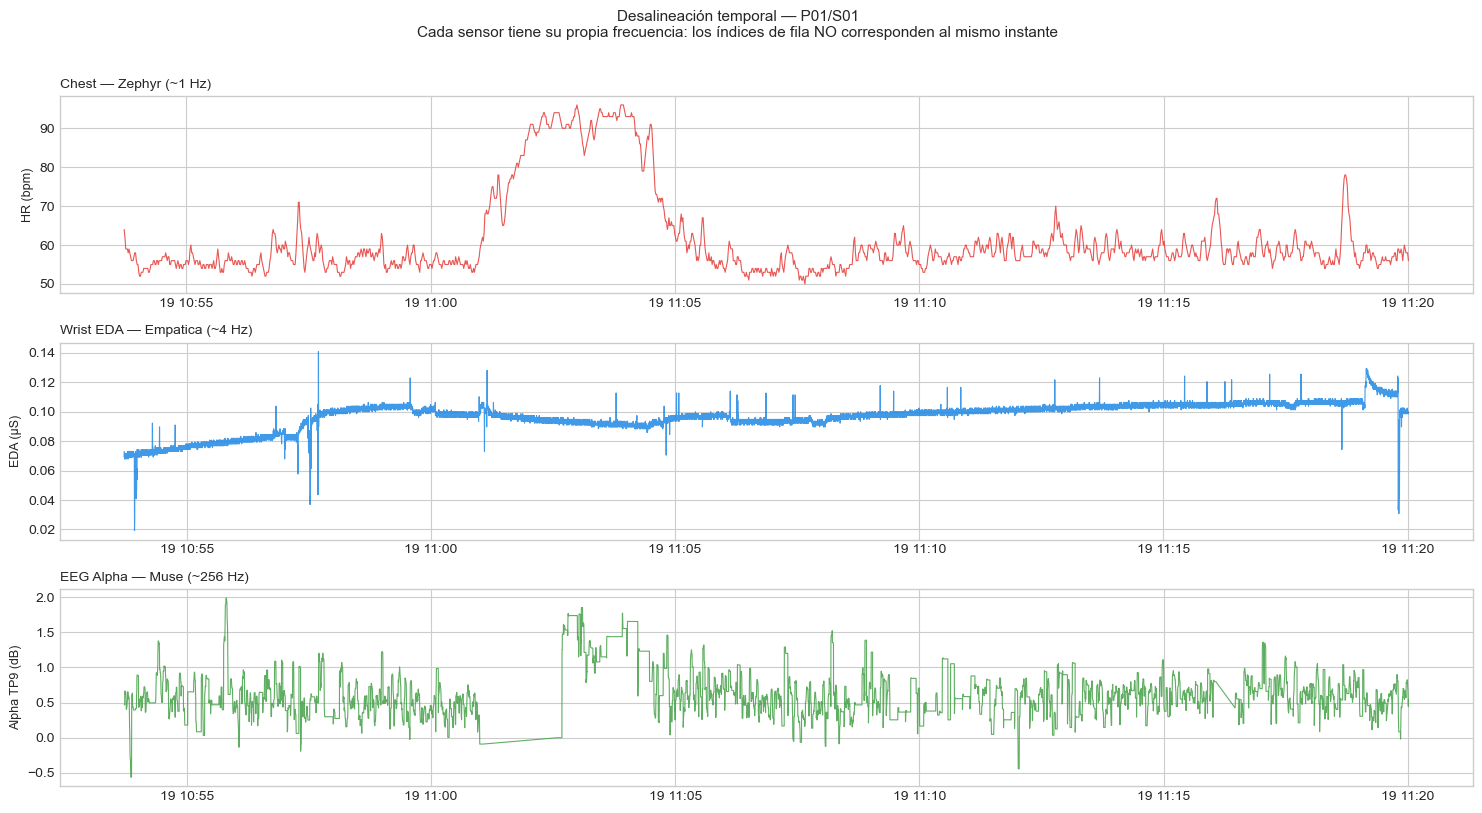
\includegraphics[width=\textwidth]{Image/Figura 1.png}
\caption{Desalineación temporal en P01/S01: cada sensor (HR, EDA, EEG) opera con su propia frecuencia y los índices de fila no representan el mismo instante.}
\label{fig:desalineacion_temporal}
\end{figure}

\subsection{Figura 2: Downsampling EDA}

\begin{figure}[H]
\centering
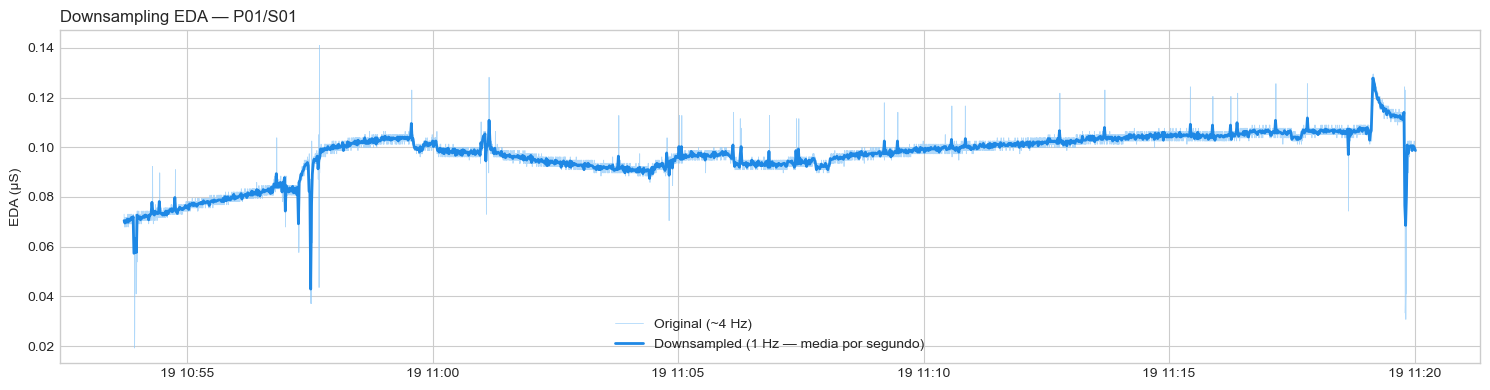
\includegraphics[width=\textwidth]{Image/Figura 2.png}
\caption{Downsampling de EDA en P01/S01: comparación entre señal original ($\sim$4 Hz) y señal agregada a 1 Hz mediante media por segundo.}
\label{fig:downsampling_eda}
\end{figure}

\subsection{Figura 3: Métodos de Interpolación}

\begin{figure}[H]
\centering
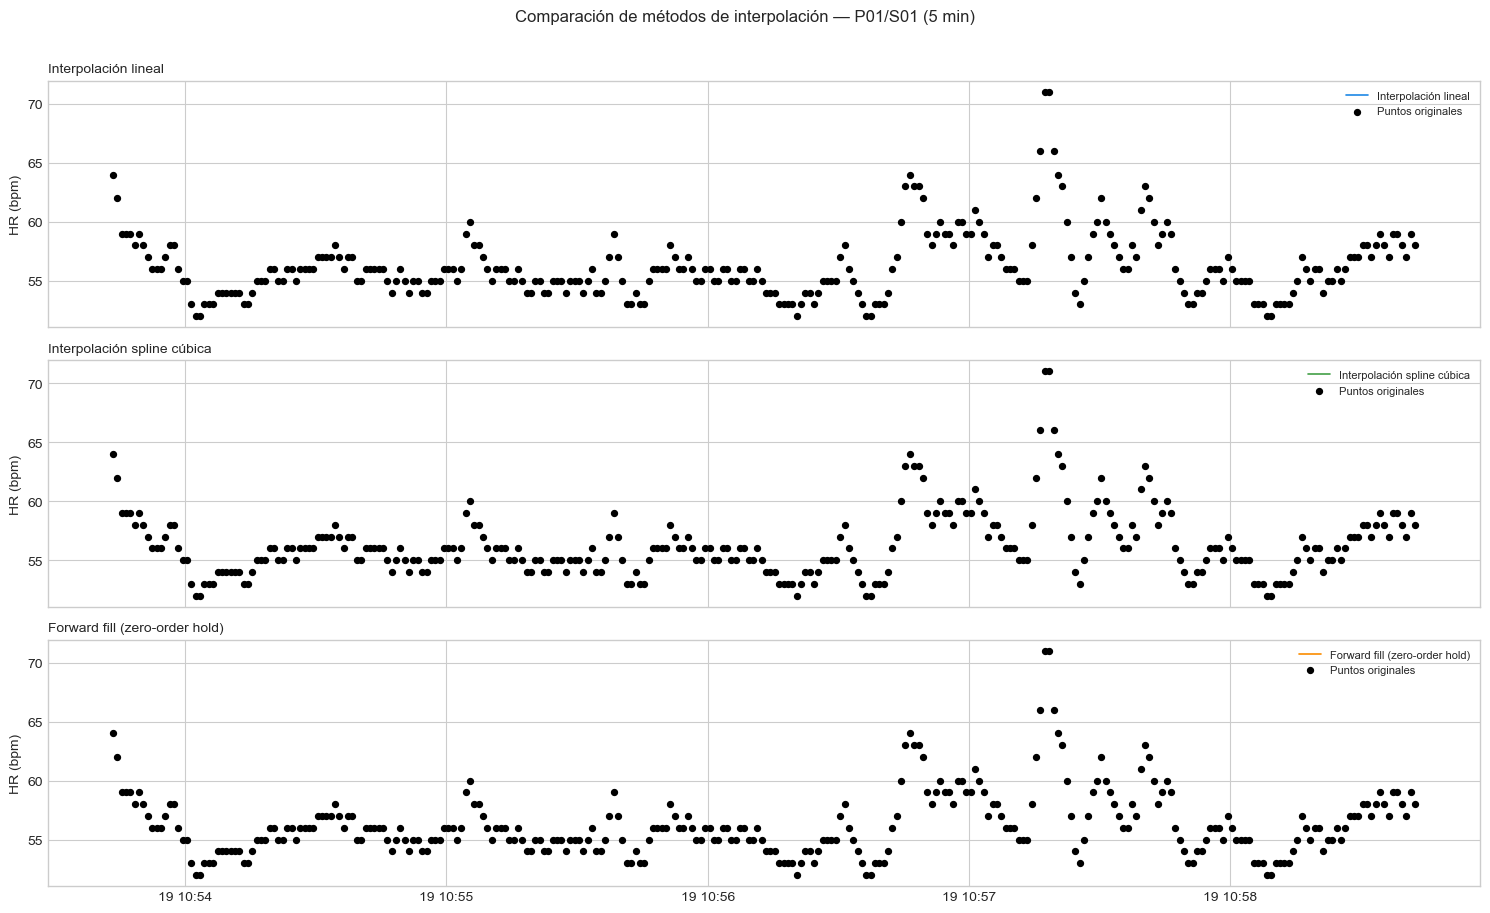
\includegraphics[width=\textwidth]{Image/Figura 3.png}
\caption{Comparación de interpolación en HR upsampled (5 minutos): lineal, spline cúbica y forward fill, junto con los puntos originales.}
\label{fig:metodos_interpolacion}
\end{figure}

\subsection{Figura 4: Tensor Sincronizado}

\begin{figure}[H]
\centering
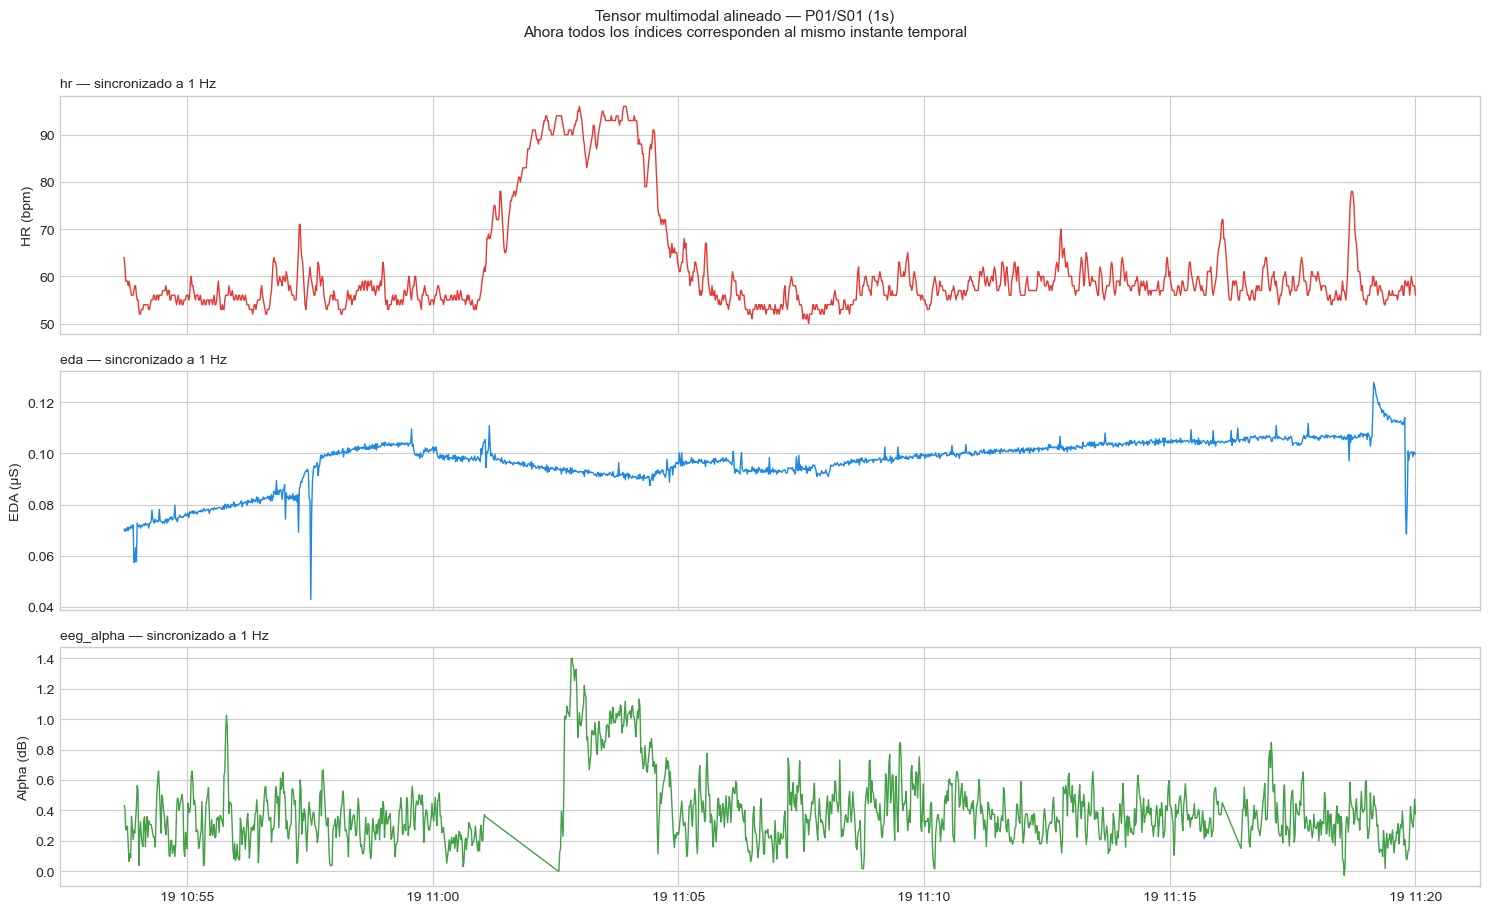
\includegraphics[width=\textwidth]{Image/Figura 4.png}
\caption{Tensor multimodal sincronizado a 1 Hz para P01/S01: HR, EDA y EEG Alpha alineados sobre un eje temporal común.}
\label{fig:tensor_sincronizado}
\end{figure}

\subsection{Figura 5: Normalización Global}

\begin{figure}[H]
\centering
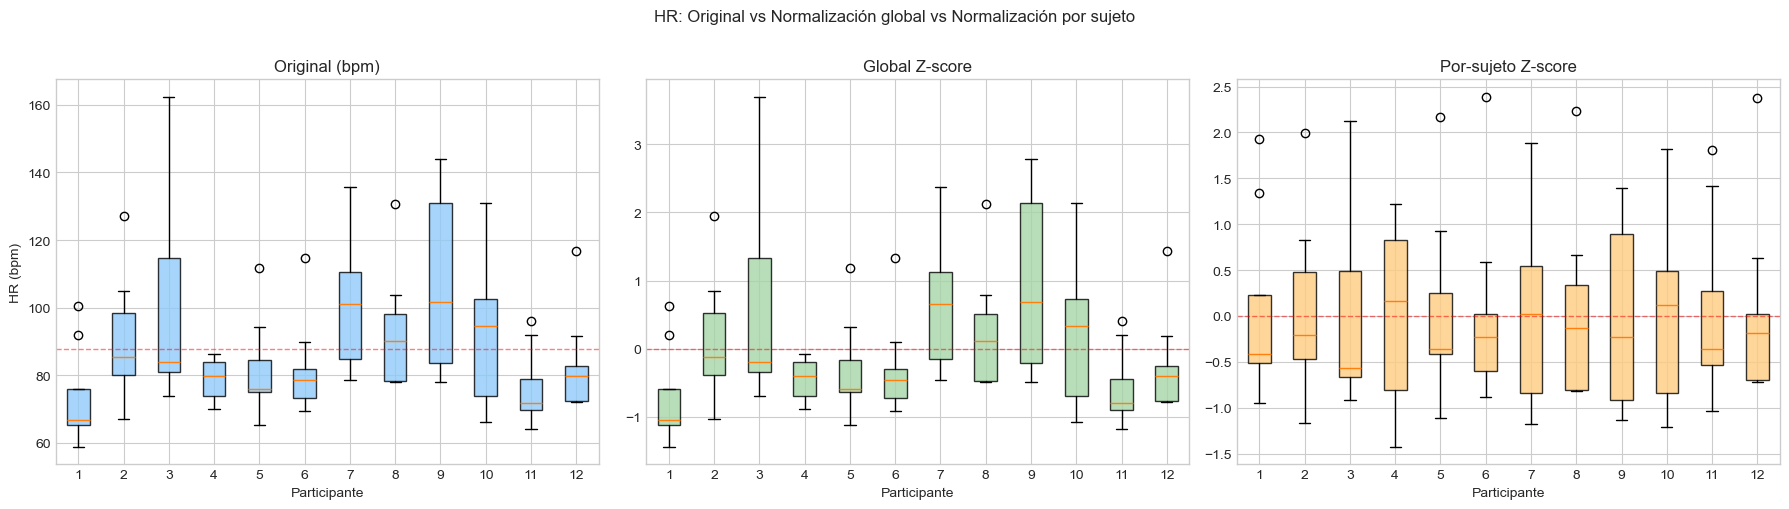
\includegraphics[width=\textwidth]{Image/Figura 5.png}
\caption{Comparación de HR original, normalización global y normalización por sujeto; se aprecia el efecto sobre la distribución por participante.}
\label{fig:normalizacion_global_vs_sujeto}
\end{figure}

\subsection{Figura 6: Split Temporal}

\begin{figure}[H]
\centering
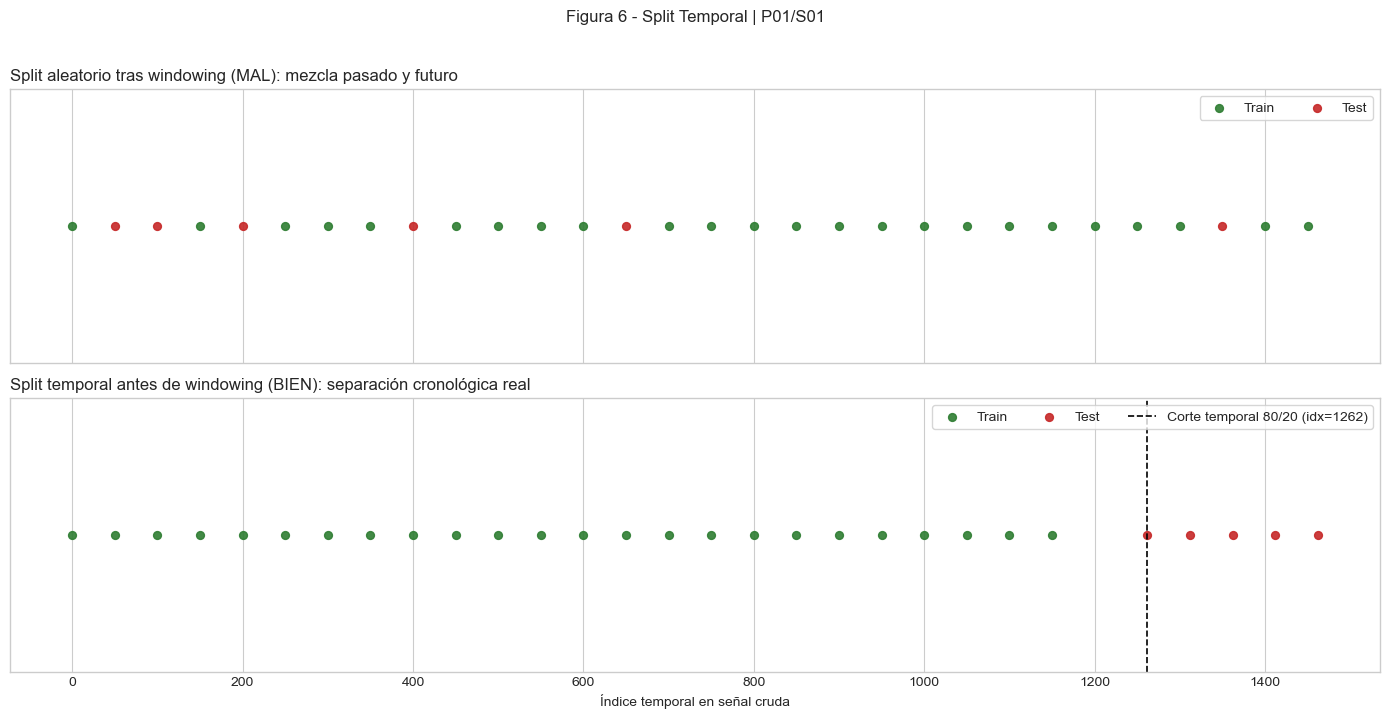
\includegraphics[width=\textwidth]{Image/Figura 6.png}
\caption{Comparación de esquemas de partición en P01/S01: split aleatorio tras windowing (incorrecto) frente a split temporal antes de windowing (correcto).}
\label{fig:split_temporal}
\end{figure}

% ============================================================
% CONCLUSIONES
% ============================================================
\newpage
\section{Conclusiones y Buenas Prácticas}

\subsection{Resumen de Operaciones}

\begin{table}[H]
\centering
\caption{Referencia rápida: técnicas y herramientas}
\label{tab:resumen_all}
\begin{tabular}{|l|l|l|}
\hline
\textbf{Técnica} & \textbf{Qué hace} & \textbf{Pandas/Scipy} \\
\hline
Windowing & Segmenta serie en bloques & \code{loop + slicing} \\
\hline
Downsampling & Reduce Hz por agregación & \code{.resample().mean()} \\
\hline
Upsampling & Aumenta Hz (crea NaN) & \code{.resample().asfreq()} \\
\hline
Interp. lineal & Rellena NaN lineal & \code{.interpolate('linear')} \\
\hline
Interp. spline & Rellena NaN curva suave & \code{.interpolate('cubic')} \\
\hline
Norm. global & Z-score todo dataset & \code{(x - x.mean())/x.std()} \\
\hline
Norm. sujeto & Z-score por persona & \code{.groupby().transform()} \\
\hline
LOSO & Validación sin leakage & Loop + recalcular $\mu/\sigma$ \\
\hline
\end{tabular}
\end{table}

\subsection{Verificación Pre-Entrenamiento}

Checklist final:

\begin{enumerate}
    \item Forma tensor: $(T, M)$ donde $T$ = instantes, $M$ = modalidades
    \item Alineación temporal: Índices $t$ corresponden al mismo instante real
    \item Sin NaN: Matriz completa después interpolación
    \item Estadísticas post-norm: $\mu \approx 0$, $\sigma \approx 1$
    \item Sin leakage temporal: Split train/test tiene frontera clara
    \item Sin leakage normalización: $\mu_{\text{norm}}, \sigma_{\text{norm}}$ solo de TRAIN
    \item LOSO para biometría: Ningún sujeto en train $\cap$ test
\end{enumerate}

\subsection{Recomendaciones para TFG}

\begin{itemize}
    \item \textbf{Priorizar LOSO}: Validación leave-one-subject-out es obligatoria en biometría

    \item \textbf{Documentar split}: Describir explícitamente temporal vs aleatorio

    \item \textbf{Reportar diagnostics}: Incluir tablas de leakage checks

    \item \textbf{Normalización conservadora}: Si dudas, usar por-sujeto para LOSO

    \item \textbf{Reproducibilidad}: Fijar random seeds, versionar scripts
\end{itemize}

\textbf{Nota importante}: Si las métricas caen después de corregir leakage, \textit{no es fracaso}. Es validez experimental recuperada.

% ============================================================
% APÉNDICE
% ============================================================
\newpage
\appendix

\section{Funciones Auxiliares}

\subsection{Similitud Coseno}

\begin{lstlisting}[caption=Similitud coseno]
import numpy as np

def cosine_similarity(u, v):
    """Similitud coseno: [-1, 1]."""
    norm_u = np.linalg.norm(u)
    norm_v = np.linalg.norm(v)

    if norm_u == 0 or norm_v == 0:
        return 0.0

    return float(np.dot(u, v) / (norm_u * norm_v))

# Ejemplo
w1 = np.array([1.2, 3.4, 5.6])
w2 = np.array([1.3, 3.3, 5.7])
sim = cosine_similarity(w1, w2)
print(f"Similitud: {sim:.4f}")  # ~0.9999
\end{lstlisting}

\subsection{Features Básicos}

\begin{lstlisting}[caption=Extracción de features estadísticos]
def calcular_features(ventana):
    """Features estadisticos de una ventana."""
    return {
        'media': float(np.mean(ventana)),
        'std': float(np.std(ventana)),
        'min': float(np.min(ventana)),
        'max': float(np.max(ventana)),
        'rango': float(np.max(ventana) - np.min(ventana)),
    }

# Ejemplo
ventana = np.array([60, 62, 61, 63, 65, 64])
feats = calcular_features(ventana)
print(feats)
\end{lstlisting}

\subsection{Validación Split Temporal}

\begin{lstlisting}[caption=Validar split temporal sin leakage]
def validar_split_temporal(df_train, df_test,
                            col_tiempo='datetime'):
    """Verifica ausencia de solapamiento temporal."""
    t_train_max = df_train[col_tiempo].max()
    t_test_min = df_test[col_tiempo].min()

    if t_test_min <= t_train_max:
        print("ERROR: Solapamiento temporal!")
        print(f"  TRAIN max: {t_train_max}")
        print(f"  TEST min: {t_test_min}")
        return False
    else:
        print("OK: Split temporal valido")
        return True
\end{lstlisting}

\section{Referencias a Notebooks}

\begin{itemize}
    \item \textbf{windowing\_data\_leakage.ipynb}:
    \begin{itemize}
        \item Análisis de leakage tipos 1-3
        \item Similitud coseno entre ventanas
        \item Comparación split aleatorio vs temporal
    \end{itemize}

    \item \textbf{sincronizacion\_normalizacion.ipynb}:
    \begin{itemize}
        \item Carga multimodal
        \item Resampling e interpolación
        \item Normalizacion global vs por-sujeto
        \item LOSO sin data leakage
    \end{itemize}
\end{itemize}

\end{document}
